\documentclass[conference]{IEEEtran}
\IEEEoverridecommandlockouts

% ============================================================
% Paquetes
% ============================================================
\usepackage[utf8]{inputenc}
\usepackage[T1]{fontenc}
\usepackage[spanish,es-tabla]{babel}
\usepackage{cite}
\usepackage{amsmath,amssymb,amsfonts}
\usepackage{graphicx}
\usepackage{booktabs}
\usepackage{tabularx}
\usepackage{subcaption}
\usepackage{textcomp}
\usepackage{xcolor}
\usepackage{listings}
\usepackage{hyperref}
\usepackage{url}

% ============================================================
% Hyperlinks
% ============================================================
\hypersetup{
    colorlinks=true,
    linkcolor=blue!60!black,
    urlcolor=blue!60!black,
    citecolor=blue!60!black,
}

% ============================================================
% Listings (código)
% ============================================================
\definecolor{codegray}{rgb}{0.95,0.95,0.95}
\definecolor{codekeyword}{rgb}{0.13,0.29,0.53}
\definecolor{codestring}{rgb}{0.31,0.60,0.02}
\definecolor{codecomment}{rgb}{0.50,0.50,0.50}

\lstset{
    backgroundcolor=\color{codegray},
    basicstyle=\ttfamily\scriptsize,
    keywordstyle=\color{codekeyword}\bfseries,
    stringstyle=\color{codestring},
    commentstyle=\color{codecomment}\itshape,
    breaklines=true,
    frame=single,
    showstringspaces=false,
    tabsize=2,
}

\def\BibTeX{{\rm B\kern-.05em{\sc i\kern-.025em b}\kern-.08em
    T\kern-.1667em\lower.7ex\hbox{E}\kern-.125emX}}

% ============================================================
% Documento
% ============================================================
\begin{document}

\title{Pregunta 03: Detección de Cumplimiento de Normas de Seguridad
en Obras de Construcción mediante YOLOv8 y Verificación Determinista
por Reglas%
\thanks{\textbf{Informe de Examen Parcial} -- Curso: Redes Neuronales y
Aprendizaje Profundo. Profesor: Ph.D.~Aldo Camargo. Universidad Nacional
de Ingeniería. Fecha de entrega: 30 de mayo de 2026.}}

\author{
    \IEEEauthorblockN{Efflyn Caja}
    \IEEEauthorblockA{
        \textit{Universidad Nacional de Ingeniería} \\
        Lima, Perú \\
        \texttt{efflyn.caja.p@uni.pe}
    }
    \and
    \IEEEauthorblockN{José Chiroques}
    \IEEEauthorblockA{
        \textit{Universidad Nacional de Ingeniería} \\
        Lima, Perú \\
        \texttt{Jchiroques@uni.pe}
    }
    \and
    \IEEEauthorblockN{Jesús Nazario}
    \IEEEauthorblockA{
        \textit{Universidad Nacional de Ingeniería} \\
        Lima, Perú \\
        \texttt{jesus.nazario.p@uni.pe}
    }
}

\maketitle

% ============================================================
% Abstract
% ============================================================
\begin{abstract}
Se presenta el diseño, implementación y mejoras iterativas de un
sistema de visión por computadora para la detección automática del
cumplimiento del casco de seguridad en obras de construcción. La
arquitectura combina un detector \textit{YOLOv8s} con un módulo
determinista de verificación por reglas, en una configuración
híbrida \emph{percepción + decisión} explícitamente requerida por el
enunciado del trabajo como criterio de calidad. El modelo, entrenado
sobre 25.976 imágenes de tres datasets públicos y posteriormente
refinado vía \textit{fine-tuning} sobre un cuarto dataset con
anotación completa, alcanza un mAP@0.5 de 0.771 sobre 3.895
imágenes de prueba no vistas, con desempeño excelente en las clases
críticas (mAP@0.5 $\geq$ 0.947). Durante el desarrollo se
identificó una limitación estructural por sesgo de etiquetado entre
datasets de origen, validada experimentalmente contra un modelo
externo que produce 2.75$\times$ más veredictos definitivos sobre la
misma escena. A partir de ese hallazgo se aplicaron dos mejoras
iterativas: un \textit{pipeline} híbrido con un detector
pre-entrenado en COCO, y un \textit{fine-tuning} sobre el dataset
\emph{Construction Site Safety} que elevó la clase \texttt{person}
desde mAP $0.176$ hasta $0.708$. El sistema se demuestra sobre dos
videos reales no vistos durante el entrenamiento.
\end{abstract}

\begin{IEEEkeywords}
detección de objetos, YOLOv8, equipos de protección personal,
seguridad ocupacional, verificación basada en reglas,
\textit{transfer learning}, \textit{fine-tuning}
\end{IEEEkeywords}

% ============================================================
\section{Introducción}
% ============================================================

\subsection{Problema}

Las obras de construcción son entornos de alto riesgo. El uso del
casco de seguridad es la medida más básica de prevención y, en el
contexto operativo peruano, la \textbf{única} universalmente
obligatoria: a diferencia de otras regiones donde el chaleco
reflectivo forma parte del uniforme estándar, en obras pequeñas y
medianas de Perú la prenda típica es polo manga larga acompañado
del casco. La supervisión manual del cumplimiento de esta norma es
costosa, intermitente y susceptible a sesgos humanos.

Este trabajo aborda tres desafíos técnicos centrales identificados
en el enunciado:
\begin{enumerate}
    \item Oclusión severa de trabajadores por maquinaria u otros
    operarios.
    \item Detección de objetos pequeños (trabajadores lejanos con
    pocos píxeles).
    \item Desbalance de clases: los casos no conformes (la clase
    crítica) son típicamente escasos en grabaciones reales.
\end{enumerate}

\subsection{Contexto operativo: regla solo-casco}
\label{sec:contexto}

Una decisión técnica central del proyecto, tomada durante el
desarrollo y descrita en la Sección~\ref{sec:decision_alcance},
fue redefinir el alcance del verificador a la regla
\textbf{solo casco}. El enunciado original mencionaba casco y
chaleco; dos factores convergieron para justificar la simplificación:
(i) realidad operativa peruana, donde el chaleco no es uniforme
universal, y (ii) limitación estructural del dataset combinado
(Sección~\ref{sec:sesgo}), donde solo el 3.3\% de las imágenes
presenta detección simultánea de cabeza y chaleco.

\subsection{Estrategia general}

Se adopta una arquitectura híbrida \emph{percepción + decisión}:
un modelo YOLOv8 realiza la percepción (detección de cabezas,
chalecos y cuerpos cuando es posible) y un módulo determinista
realiza la decisión (veredicto por trabajador). Esta separación es
un requisito explícito del enunciado y favorece la auditabilidad y
modificabilidad sin reentrenar el modelo.

% ============================================================
\section{Datos}
% ============================================================

\subsection{Fuentes}

Se combinaron tres datasets públicos de Roboflow Universe
\cite{roboflow} en formato YOLOv8 (Tabla~\ref{tab:datasets}). Un
cuarto dataset, \emph{Construction Site Safety}, se incorporó
posteriormente para el \textit{fine-tuning}
(Sección~\ref{sec:finetuning}).

\begin{table}[h]
\centering
\caption{Datasets de origen combinados.}
\label{tab:datasets}
\renewcommand{\arraystretch}{1.15}
\begin{tabular}{l r}
\toprule
\textbf{Dataset} & \textbf{Imágenes} \\
\midrule
Hard Hat Workers (Northeastern) & 7.035 \\
Safety Helmet (lisa-group-de) & 7.035 \\
Safety Vest PPE & 11.906 \\
\midrule
\textbf{Total corpus principal} & \textbf{25.976} \\
\midrule
Construction Site Safety (OtroEnfoque) & 2.719 \\
\bottomrule
\end{tabular}
\end{table}

\subsection{Taxonomía unificada}

Las clases originales se remapearon a una taxonomía común de cinco
clases mediante una tabla declarativa versionada en
\texttt{configs/class\_mapping.yaml}:

\begin{table}[h]
\centering
\caption{Taxonomía unificada de 5 clases.}
\label{tab:taxonomia}
\renewcommand{\arraystretch}{1.15}
\begin{tabular}{c l}
\toprule
\textbf{id} & \textbf{Clase} \\
\midrule
0 & head\_with\_helmet \\
1 & head\_without\_helmet \\
2 & person \\
3 & vest \\
4 & no\_vest\_person \\
\bottomrule
\end{tabular}
\end{table}

\subsection{Splits estratificados}

Se generaron splits 70/15/15 train/val/test estratificados por
\emph{combinación de clases presentes en cada imagen}, lo que
preserva la proporción de cada clase en cada split y previene la
fuga de datos. La Figura~\ref{fig:dist} muestra la distribución
resultante.

\begin{figure}[h]
\centering
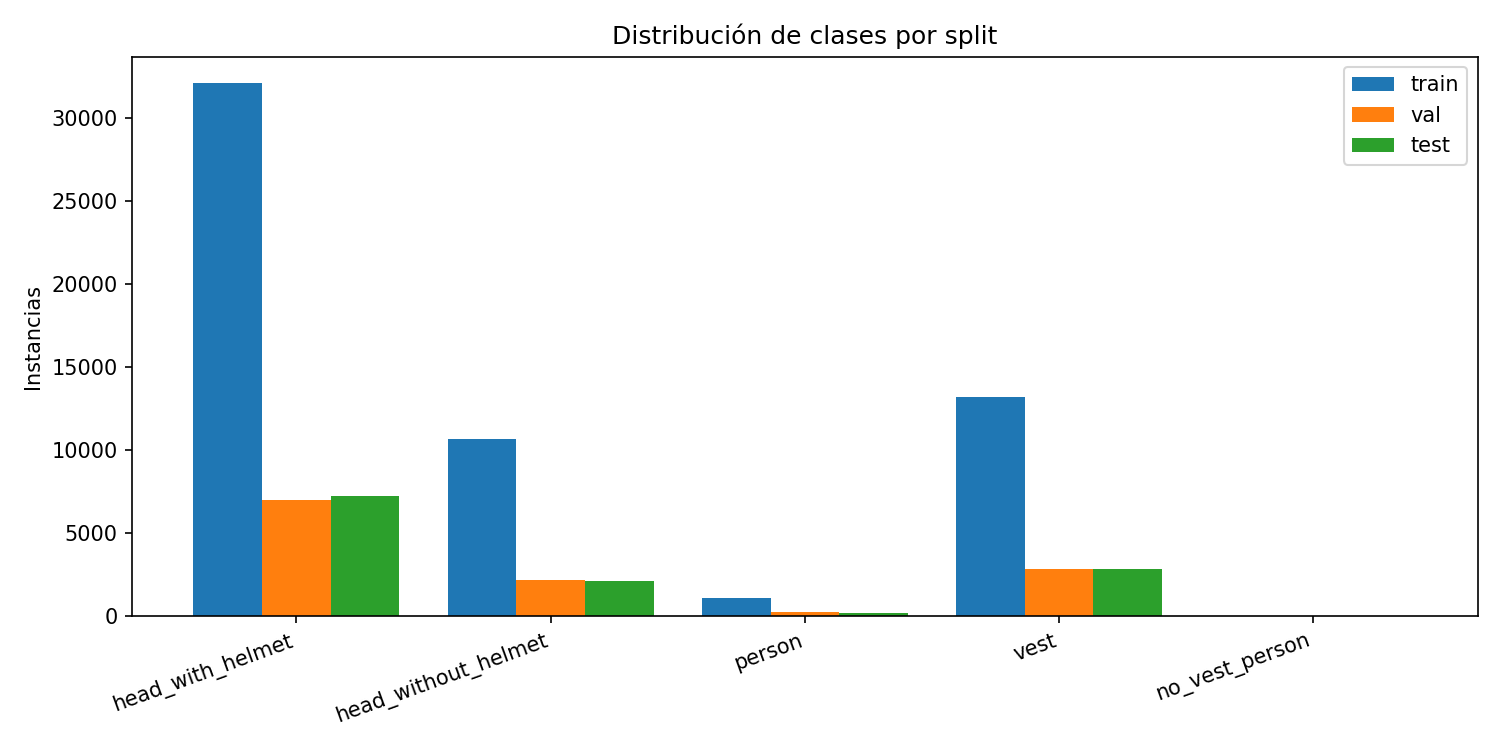
\includegraphics[width=0.95\columnwidth]{figures/class_distribution.png}
\caption{Distribución de instancias por clase y por split. La clase
\texttt{person} representa solo el 2\% del total (1.116 train), lo
que motivará una mejora iterativa.}
\label{fig:dist}
\end{figure}

\subsection{Reconocimiento de límites}

Se identifican tres limitaciones explícitas: (i) \texttt{person}
muy escasa (2\% de las instancias), (ii) \texttt{no\_vest\_person}
ausente, inferida por reglas espaciales en el verificador, y
(iii) anotación parcial no superpuesta entre los tres datasets,
discutida en profundidad en la Sección~\ref{sec:sesgo}.

% ============================================================
\section{Metodología}
% ============================================================

\subsection{Elección del modelo}

Se eligió YOLOv8 \cite{ultralytics2023} (Ultralytics, versión 8.x)
por madurez del \emph{tooling}, documentación extensa,
compatibilidad probada con Kaggle y excelente relación
costo-beneficio frente a YOLOv9 para un parcial con plazo definido.
Se usó la variante YOLOv8s ($\sim$11M parámetros), que entra cómoda
en la VRAM de una GPU T4 con \textit{batch size} 16.

\subsection{Configuración del baseline}

\begin{table}[h]
\centering
\caption{Hiperparámetros del baseline.}
\label{tab:hyp}
\renewcommand{\arraystretch}{1.1}
\begin{tabular}{l l}
\toprule
\textbf{Hiperparámetro} & \textbf{Valor} \\
\midrule
Resolución de entrada & 640$\times$640 \\
Epochs & 80 \\
\textit{Patience} (\textit{early stopping}) & 20 \\
Optimizador & SGD \\
\textit{Learning rate} inicial & 0.01 \\
\textit{Batch size} & 16 \\
Mosaic & 1.0 \\
MixUp / Random Erasing & 0.0 \\
\bottomrule
\end{tabular}
\end{table}

\subsection{Experimentos comparativos}

Se diseñaron cuatro experimentos. Por restricciones de cuota GPU en
Kaggle (30~h semanales, $\sim$7-8~h por entrenamiento) se
ejecutaron dos. Los descartes se justifican:

\begin{itemize}
    \item \textbf{Experimento A descartado}: resolución 960 estimaba
    12-15~h, sobre el límite de 12~h por sesión.
    \item \textbf{Experimento C descartado}: el problema de
    \texttt{person} es de \emph{cantidad de datos} (1.116 train),
    no de balance. Ningún esquema de pesos inventa más ejemplos.
    Este diagnóstico se valida posteriormente
    (Sección~\ref{sec:finetuning}).
\end{itemize}

\subsection{Decisiones técnicas}

\textbf{Anchors:} YOLOv8 usa estrategia \emph{anchor-free} con
Distribution Focal Loss; no hay anchors a configurar.
\textbf{Augmentaciones:} estrictamente las nativas de Ultralytics.
El Exp. B añadió Random Erasing y MixUp moderado.
\textbf{Mosaic:} activo durante 65 de 80 epochs en el modelo final
(\texttt{close\_mosaic=15}).

% ============================================================
\section{Resultados cuantitativos}
% ============================================================

\subsection{Comparación de experimentos sobre validación}

\begin{table}[h]
\centering
\caption{Comparación de experimentos sobre val. Modelo elegido:
Experimento D.}
\label{tab:cmp_val}
\renewcommand{\arraystretch}{1.15}
\begin{tabular}{l rrr}
\toprule
\textbf{Clase} & \textbf{Baseline} & \textbf{Exp B} & \textbf{Exp D} \\
\midrule
head\_with\_helmet & 0.978 & 0.978 & \textbf{0.979} \\
head\_without\_helmet & 0.959 & 0.960 & 0.959 \\
vest & 0.987 & 0.986 & 0.986 \\
person & 0.175 & 0.153 & 0.175 \\
\midrule
\textbf{all mAP@0.5} & \textbf{0.775} & 0.769 & \textbf{0.775} \\
\textbf{all mAP@0.5--0.95} & 0.567 & 0.562 & \textbf{0.569} \\
\bottomrule
\end{tabular}
\end{table}

\textbf{Hallazgo del Exp. B}: las augmentaciones agresivas no
aportaron mejora; degradaron 0.6~pp la precisión global. El dataset
ya contenía suficiente variabilidad natural.

\subsection{Evaluación sobre test set}

\begin{table*}[t]
\centering
\caption{Métricas finales del modelo D sobre el test set (3.895
imágenes nunca vistas).}
\label{tab:test}
\renewcommand{\arraystretch}{1.2}
\begin{tabular}{l rrrrr}
\toprule
\textbf{Clase} & \textbf{Inst.} & \textbf{Precision} & \textbf{Recall}
& \textbf{mAP@0.5} & \textbf{mAP@0.5--0.95} \\
\midrule
head\_with\_helmet & 7.222 & 0.939 & 0.950 & \textbf{0.976} & 0.664 \\
head\_without\_helmet & 2.104 & 0.892 & 0.942 & \textbf{0.947} & 0.646 \\
vest & 2.831 & 0.937 & 0.957 & \textbf{0.984} & 0.837 \\
person & 216 & 0.341 & 0.208 & 0.176 & 0.129 \\
\midrule
\textbf{all} & 12.373 & \textbf{0.777} & \textbf{0.765} & \textbf{0.771} & \textbf{0.569} \\
\bottomrule
\end{tabular}
\end{table*}

\begin{figure}[h]
\centering
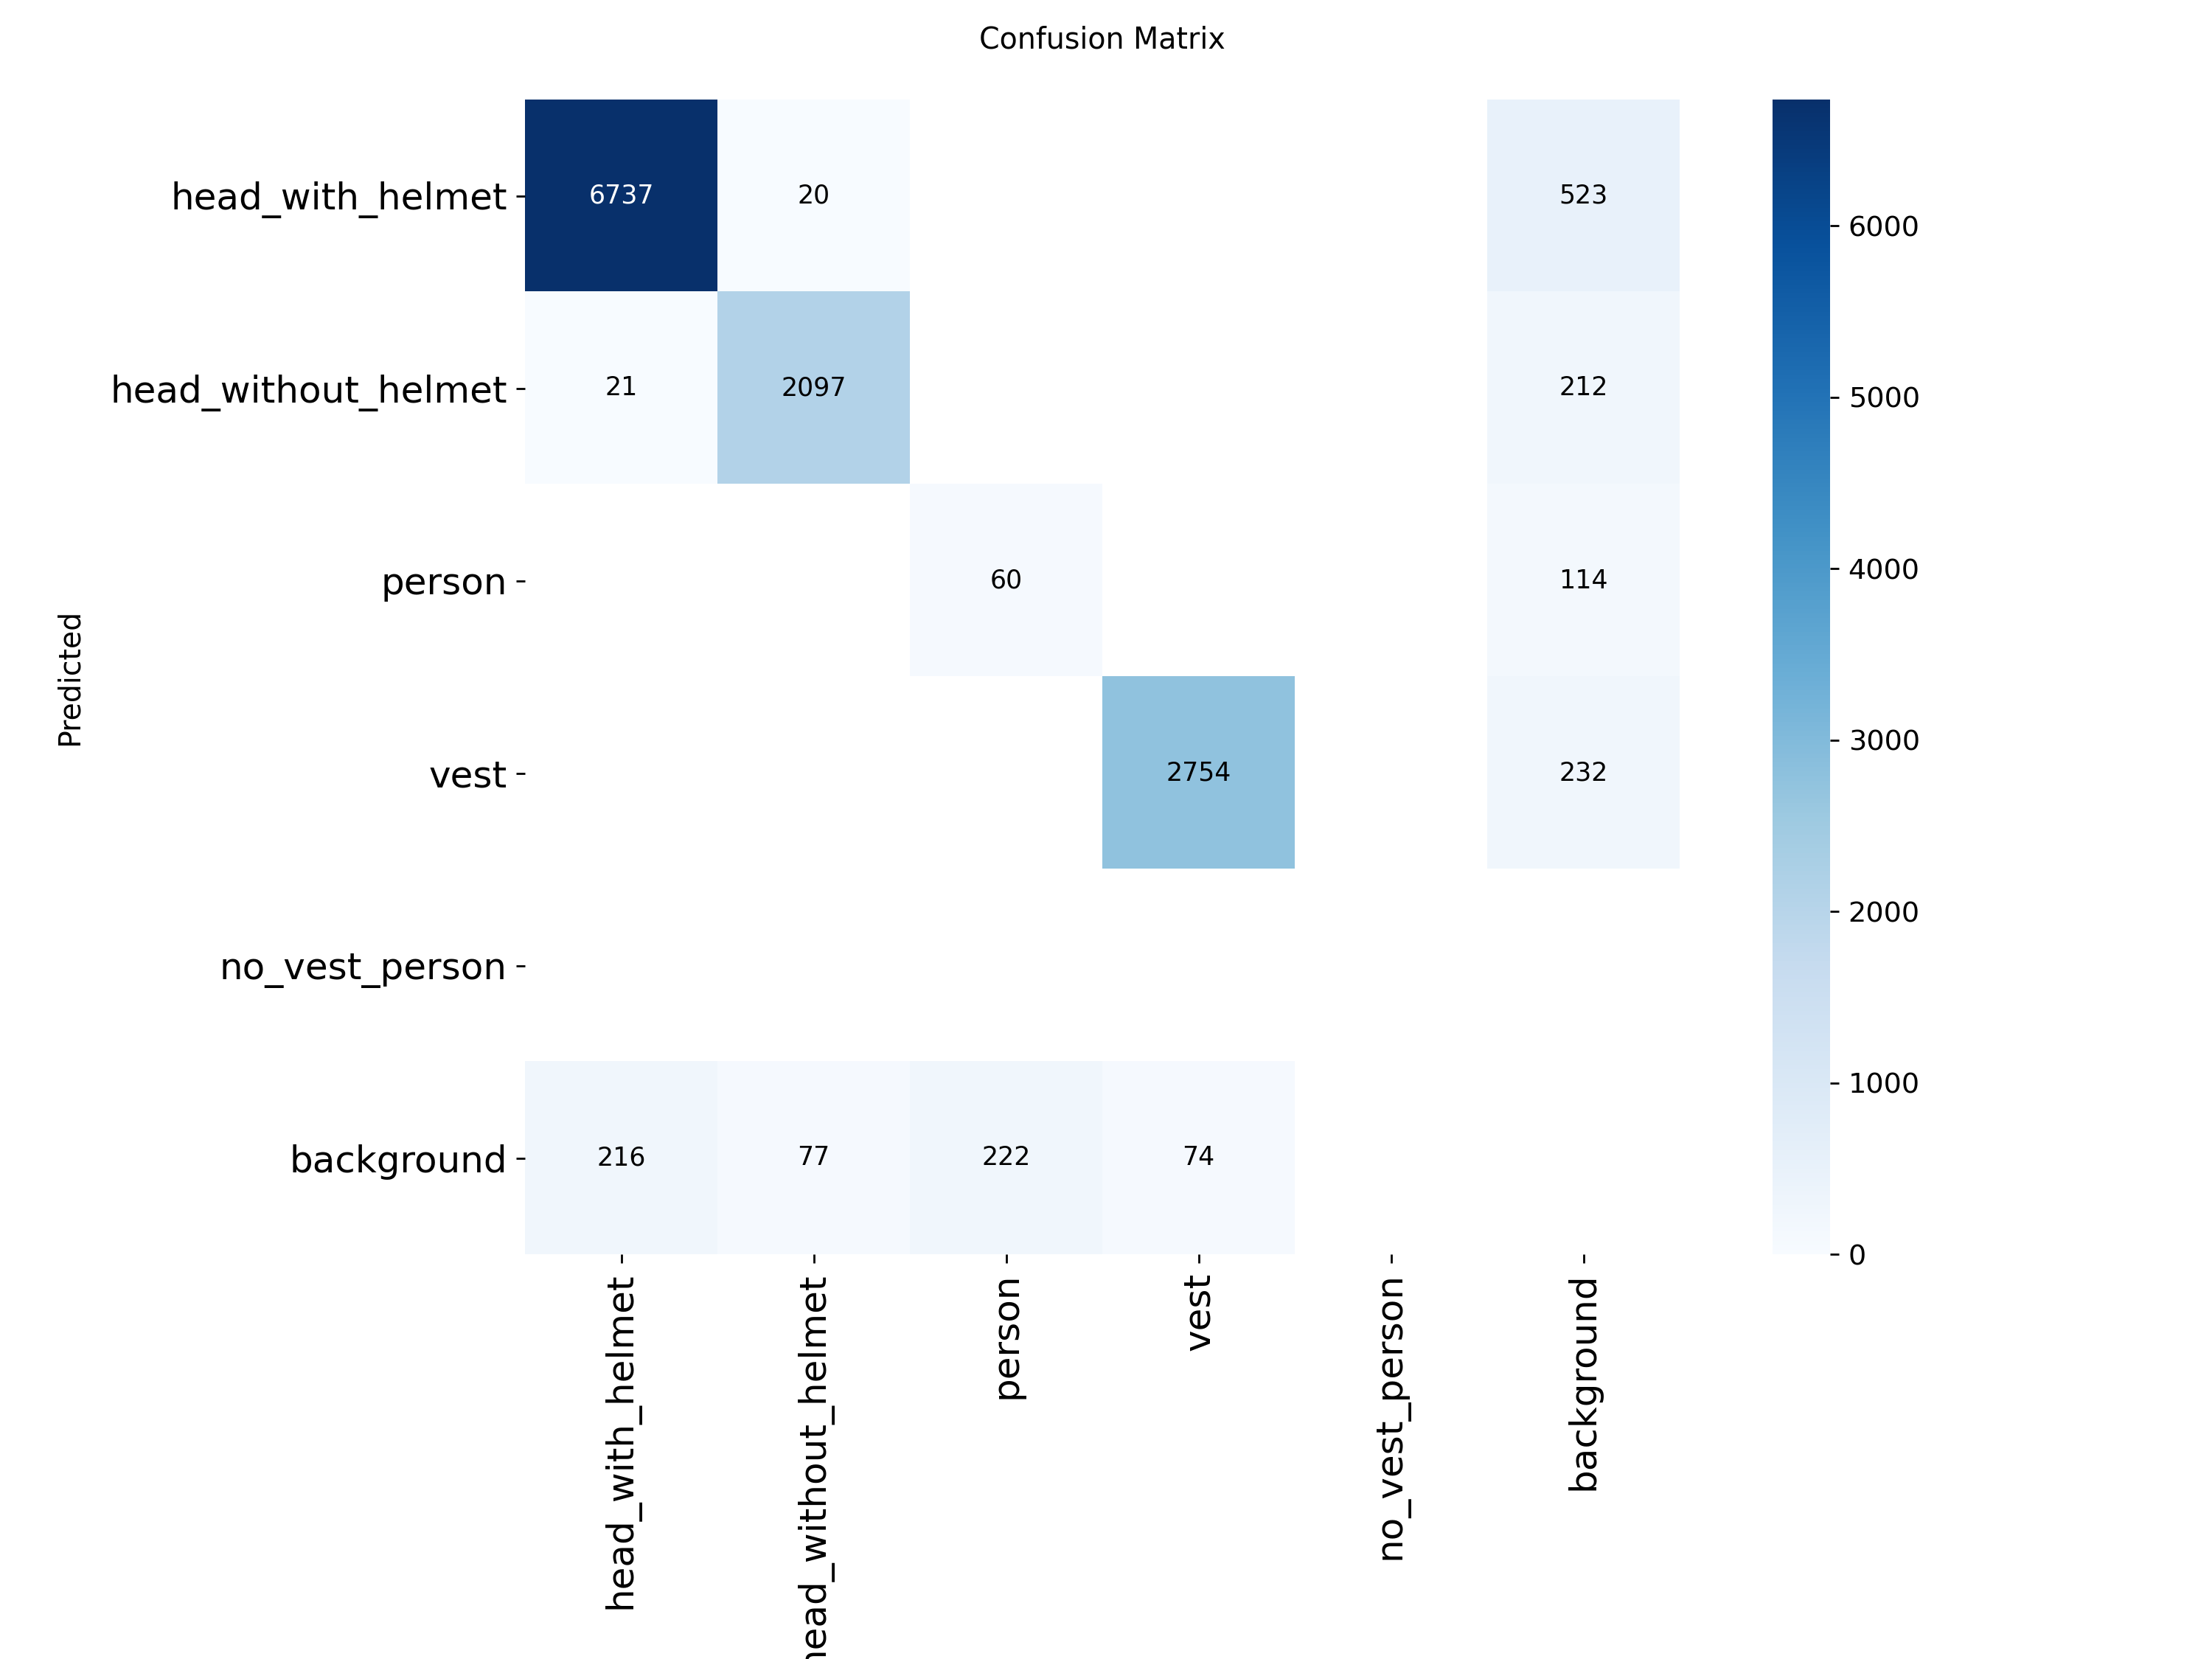
\includegraphics[width=0.85\columnwidth]{figures/confusion_exp_D.png}
\caption{Matriz de confusión del modelo D sobre validación. Diagonal
fuerte para las tres clases principales y confusión inexistente
entre clases.}
\label{fig:cm}
\end{figure}

\subsection{Generalización (val vs test)}

Las métricas test son prácticamente idénticas a las de val
($\Delta$mAP@0.5 = $-0.004$), confirmando que el modelo
\textbf{no presenta overfitting} y que los splits estratificados sin
fuga funcionaron correctamente.

\subsection{Análisis de robustez por nivel de oclusión}

Para cada imagen del test se calculó el IoU máximo entre cualquier
par de cajas anotadas, clasificándola en tres niveles (bajo $<0.15$,
medio $[0.15,0.40)$, alto $\geq0.40$):

\begin{table}[h]
\centering
\caption{Métricas por nivel de oclusión sobre el test set.}
\label{tab:occ}
\renewcommand{\arraystretch}{1.15}
\begin{tabular}{l r r r}
\toprule
\textbf{Nivel} & \textbf{n} & \textbf{mAP@0.5} & \textbf{Recall} \\
\midrule
Bajo & 3.695 & 0.779 & 0.796 \\
Medio & 185 & 0.789 & 0.749 \\
Alto & 15 & 0.704 & 0.623 \\
\midrule
\textbf{Caída bajo $\to$ alto} & — & \textbf{$-7.5$~pp} & \textbf{$-17.3$~pp} \\
\bottomrule
\end{tabular}
\end{table}

\textbf{Lectura}: el modelo es robusto a oclusión leve-media. La
oclusión alta degrada principalmente el recall ($-17.3$~pp), no la
precisión ($+0.1$~pp): el modelo \emph{pierde detecciones} cuando
hay oclusión fuerte, no las \emph{inventa}. Es el comportamiento
más conservador para seguridad. \textbf{Caveat estadístico}: el
grupo ``alto'' tiene $n=15$.

% ============================================================
\section{Verificador determinista}
% ============================================================

\subsection{Diseño}

El verificador es un módulo Python independiente
(\texttt{src/compliance/}) con tres archivos: \texttt{geometry.py}
(utilidades puras), \texttt{verifier.py} (lógica de decisión) y
\texttt{renderer.py} (rendering con Supervision). Cuenta con 39
tests unitarios pytest pasando.

\subsection{Estrategia cabeza-ancla}

El diseño inicial usaba \texttt{person} como ancla. En evaluación
cualitativa este diseño falló porque la clase \texttt{person} tiene
\emph{recall} del 17\% sobre val. Se reescribió la lógica como
\emph{cabeza-ancla}: para cada cabeza detectada se busca veredicto
inmediato; si existe una detección \texttt{person} que contenga la
cabeza, se usa para enriquecer el rendering.

\subsection{Decisión de alcance: regla solo-casco}
\label{sec:decision_alcance}

Tras diagnosticar el sesgo de datasets (Sección~\ref{sec:sesgo}) y
considerar el contexto operativo (Sección~\ref{sec:contexto}), se
adoptó la regla \textbf{solo-casco}:

\begin{table}[h]
\centering
\caption{Lógica del verificador (regla solo-casco).}
\label{tab:logica}
\renewcommand{\arraystretch}{1.15}
\begin{tabular}{p{3.5cm} l}
\toprule
\textbf{Detección} & \textbf{Veredicto} \\
\midrule
Cabeza con casco & \textbf{CONFORME} \\
Cabeza sin casco & NO\_CONFORME (casco\_ausente) \\
Persona sin cabeza visible & INDETERMINADO (cabeza\_no\_visible) \\
Chaleco / no\_vest\_person & (ignorado) \\
\bottomrule
\end{tabular}
\end{table}

La separación de INDETERMINADO de NO\_CONFORME es deliberada: solo
se penaliza cuando hay evidencia explícita de falta, no cuando
simplemente no se ve la cabeza del trabajador.

\subsection{Núcleo del verificador}

\begin{lstlisting}[language=Python, basicstyle=\ttfamily\scriptsize]
def verify_frame(detections, cfg=None):
    cfg = cfg or VerifierConfig()
    heads_helmet, heads_no_helmet, persons = \
        _split_by_class(detections)
    all_heads = [(h, CLASS_HEAD_WITH_HELMET)
                 for h in heads_helmet] + \
                [(h, CLASS_HEAD_WITHOUT_HELMET)
                 for h in heads_no_helmet]

    verdicts = []
    for head, head_class in all_heads:
        person_det = _find_person_for_head(head, persons)
        if head_class == CLASS_HEAD_WITH_HELMET:
            status = ComplianceStatus.CONFORME
            reasons = []
        else:
            status = ComplianceStatus.NO_CONFORME
            reasons = ["casco_ausente"]
        bbox = person_det.box if person_det else \
               _virtual_worker_bbox(head)
        verdicts.append(PersonVerdict(...))

    # INDETERMINADO por persona sin cabeza
    for person in persons:
        if any(_head_inside_person(h, person)
               for h, _ in all_heads):
            continue
        verdicts.append(PersonVerdict(
            person_box=person.box,
            status=ComplianceStatus.INDETERMINADO,
            reasons=["cabeza_no_visible"]))

    return FrameReport(verdicts=verdicts,
                       compliance_rate=rate)
\end{lstlisting}

\begin{figure}[h]
\centering
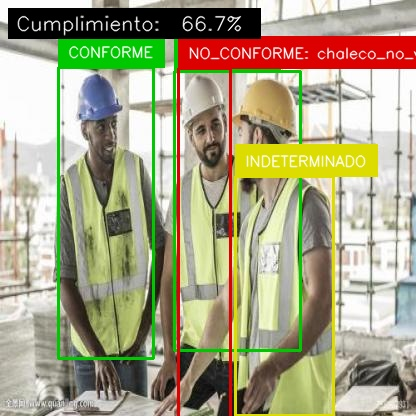
\includegraphics[width=0.85\columnwidth]{figures/verifier_imagen.jpg}
\caption{Salida del verificador sobre una imagen de validación: 3
trabajadores detectados (CONFORME / NO\_CONFORME / INDETERMINADO).
Tasa de cumplimiento del fotograma: 66.7\%.}
\end{figure}

% ============================================================
\section{Hallazgo principal: sesgo de etiquetado}
\label{sec:sesgo}
% ============================================================

\subsection{Diagnóstico cuantitativo}

Sobre 300 imágenes val analizadas con el modelo D, solo el
\textbf{3.3\%} tiene cabeza y chaleco detectados simultáneamente
(49\% solo cabeza, 40.3\% solo chaleco). La causa es estructural:
SHWD \cite{shwd} y Hard Hat anotan solo cabezas; PPE anota solo
chalecos. El modelo aprendió la correlación ``estilo de imagen
$\to$ clases visibles'' y se comporta de manera bimodal.

\subsection{Validación experimental con modelo externo}

Para verificar si la limitación era del \emph{pipeline} o del
\emph{modelo}, se ejecutó el mismo \emph{pipeline} sustituyendo
el modelo D por un modelo externo entrenado sobre un dataset con
anotación completa por trabajador. El verificador y el renderer
no se modificaron.

\begin{table}[h]
\centering
\caption{Validación experimental sobre el mismo video.}
\label{tab:validacion}
\renewcommand{\arraystretch}{1.15}
\begin{tabular}{l r r r}
\toprule
\textbf{Métrica} & \textbf{D} & \textbf{Externo} & \textbf{Ratio} \\
\midrule
CONFORME & 861 & 2.287 & $2.66\times$ \\
NO\_CONFORME & 2.600 & 7.221 & $2.78\times$ \\
INDETERMINADO & 1.309 & 397 & $0.30\times \downarrow$ \\
Veredictos definitivos & 3.461 & 9.508 & \textbf{$2.75\times$} \\
\bottomrule
\end{tabular}
\end{table}

\textbf{Conclusión}: el cuello de botella es el dataset combinado,
no el \emph{pipeline}.

% ============================================================
\section{Mejora iterativa I: pipeline híbrido}
% ============================================================

\subsection{Principio guía}

\begin{quotation}
\textit{``Si para el ojo humano es evidente ver el casco, para la
IA también debería serlo. Pero si para el ojo humano se dificulta,
ahí recién la IA podría desvariar.''}
\end{quotation}

Este principio de \emph{calibración con observador humano} motivó
la primera mejora.

\subsection{Implementación}

El \textit{pipeline} combina dos modelos:
\begin{enumerate}
    \item Modelo D (nuestro): solo cabezas.
    \item YOLOv8s pre-entrenado en COCO \cite{cocometrics}: solo
    \texttt{person} (clase 0 de COCO).
\end{enumerate}

Las detecciones se concatenan y se pasan al verificador. \textbf{El
verificador no se modifica.}

\subsection{Resultados}

El \emph{pipeline} híbrido eliminó los \emph{frames vacíos} en
escenas donde un humano sí vería al trabajador, pasando de 3 a
2.306 detecciones INDETERMINADO sobre el video03 (incremento de
cobertura $1.67\times$).

% ============================================================
\section{Mejora iterativa II: fine-tuning sobre OtroEnfoque}
\label{sec:finetuning}
% ============================================================

\subsection{Motivación y decisión}

El \textit{pipeline} híbrido resuelve cobertura pero requiere dos
modelos en paralelo. Se opta por \textbf{fine-tuning sobre
OtroEnfoque}, no por reentrenamiento desde cero, para mantener la
autoría del modelo y preservar el conocimiento adquirido sobre
casco. El dataset OtroEnfoque aporta 9.698 instancias de
\texttt{person}, ocho veces más que el corpus original.

\subsection{Configuración}

\begin{lstlisting}[language=Python, basicstyle=\ttfamily\scriptsize]
model = YOLO(WEIGHTS)  # best.pt del modelo D

results = model.train(
    data=str(patched),
    name="finetune_otroenfoque",
    epochs=25,
    patience=10,
    imgsz=640,
    batch=16,
    optimizer="SGD",
    lr0=0.001,        # 10x menor que original
    lrf=0.01,
    momentum=0.937,
    warmup_epochs=2.0,
    mosaic=1.0,
    mixup=0.0,
    erasing=0.0,
    close_mosaic=8,
    fliplr=0.5,
)
\end{lstlisting}

El \textit{learning rate} reducido (0.001 vs 0.01 original) busca
evitar \emph{catastrophic forgetting}: el modelo se ajusta sin
destruir lo aprendido. Tiempo total: 40 minutos en GPU T4.

\subsection{Resultados}

\begin{table}[h]
\centering
\caption{Métricas del modelo fine-tuned sobre val de OtroEnfoque.}
\label{tab:finetuned}
\renewcommand{\arraystretch}{1.15}
\begin{tabular}{l r r}
\toprule
\textbf{Clase} & \textbf{mAP@0.5} & \textbf{mAP@0.5-0.95} \\
\midrule
head\_with\_helmet & 0.733 & 0.435 \\
head\_without\_helmet & 0.551 & 0.285 \\
\textbf{person} & \textbf{0.708} & \textbf{0.473} \\
vest & 0.643 & 0.395 \\
no\_vest\_person & 0.588 & 0.326 \\
\midrule
\textbf{all} & \textbf{0.645} & \textbf{0.383} \\
\bottomrule
\end{tabular}
\end{table}

\textbf{Hallazgo principal}: la clase \texttt{person} saltó de
$0.176$ a $0.708$ en mAP@0.5 ($+302\%$ relativo). La clase
\texttt{no\_vest\_person}, antes inexistente, ahora opera con mAP
$0.588$.

% ============================================================
\section{Demostración en video}
% ============================================================

\subsection{Material y configuración}

Se procesaron dos videos de obras reales no vistos durante el
entrenamiento: \texttt{video03p.mp4} (cuadrilla colombiana
vertiendo concreto, plano cercano, 25.8~s a 30~fps,
1920$\times$1080) y \texttt{video04.mp4} (panorámico portuario,
19.8~s, 3842$\times$2160 4K). Configuración: \textit{resolución de
inferencia} 1280, \textit{umbral de confianza} 0.15.

\subsection{Comparación de las tres versiones}

\begin{table}[h]
\centering
\caption{Veredictos sobre \texttt{video03p.mp4} (773 frames).}
\label{tab:video03}
\renewcommand{\arraystretch}{1.15}
\begin{tabular}{l r r r}
\toprule
\textbf{Métrica} & \textbf{D solo} & \textbf{Híbrido} & \textbf{Fine-t.} \\
\midrule
CONFORME & 3.461 & 3.461 & \textbf{6.594} \\
NO\_CONFORME & 0 & 0 & 122 \\
INDETERMINADO & 3 & 2.306 & 896 \\
\% definitivos & 99.9\% & 60\% & 88\% \\
\bottomrule
\end{tabular}
\end{table}

\begin{table}[h]
\centering
\caption{Veredictos sobre \texttt{video04.mp4} panorámico 4K
(593 frames).}
\label{tab:video04}
\renewcommand{\arraystretch}{1.15}
\begin{tabular}{l r r r}
\toprule
\textbf{Métrica} & \textbf{D solo} & \textbf{Híbrido} & \textbf{Fine-t.} \\
\midrule
CONFORME & 85 & 2.287 & \textbf{7.669} \\
NO\_CONFORME & 0 & 0 & 106 \\
INDETERMINADO & 7.015 & 6.871 & 1.937 \\
\% definitivos & 1.2\% & 25\% & \textbf{80\%} \\
\bottomrule
\end{tabular}
\end{table}

\begin{figure*}[t]
\centering
\begin{subfigure}{0.32\textwidth}
    \centering
    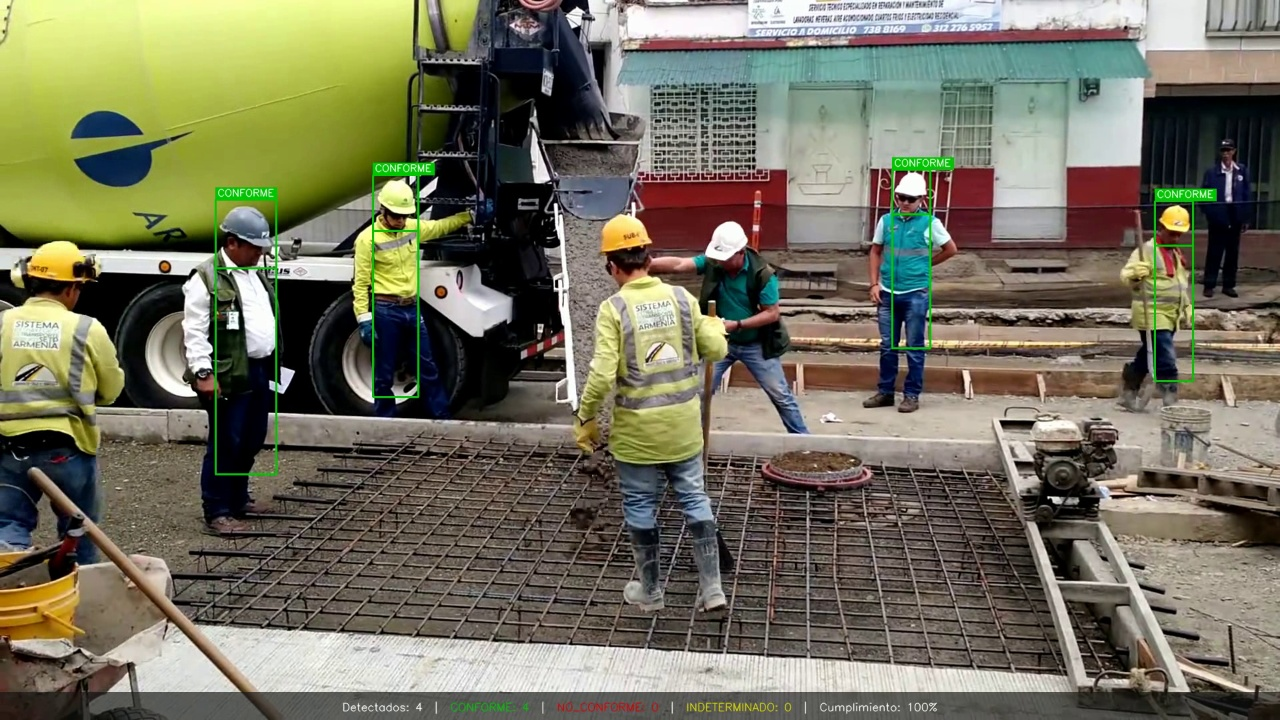
\includegraphics[width=\linewidth]{figures/demo_solo_casco.jpg}
    \caption{Modelo D solo}
\end{subfigure}
\hfill
\begin{subfigure}{0.32\textwidth}
    \centering
    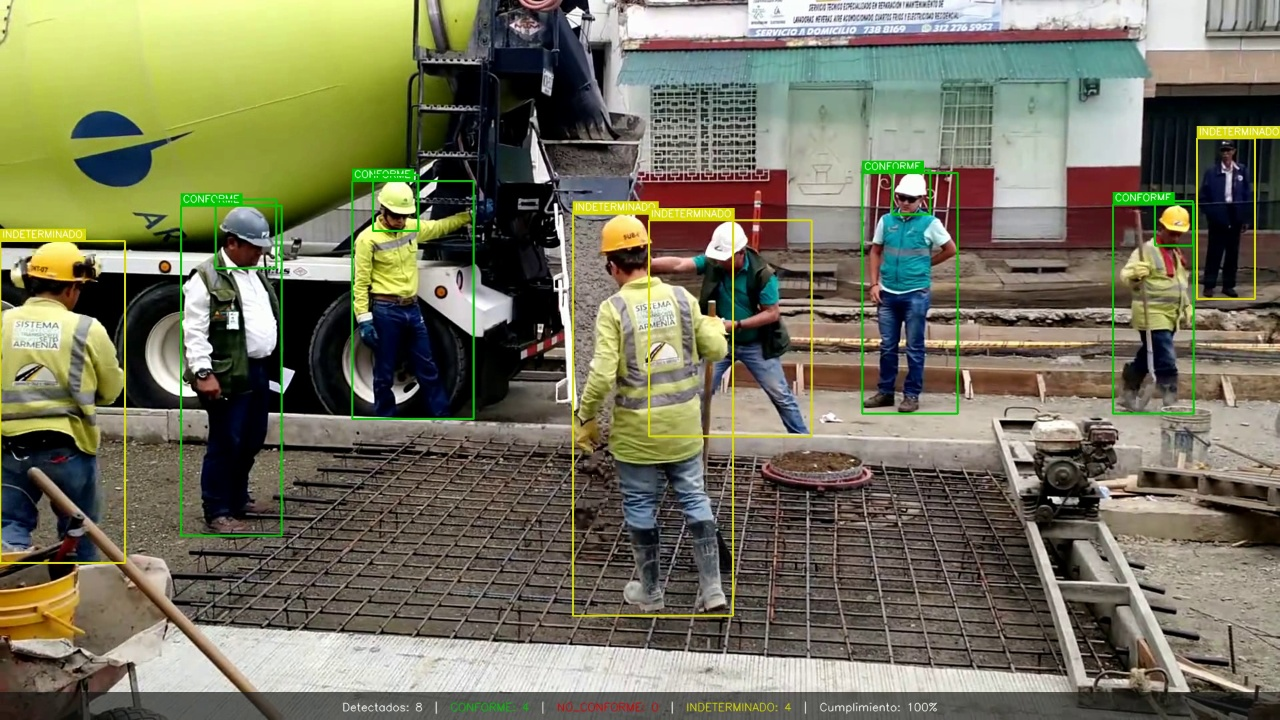
\includegraphics[width=\linewidth]{figures/demo_hibrido.jpg}
    \caption{Híbrido D+COCO}
\end{subfigure}
\hfill
\begin{subfigure}{0.32\textwidth}
    \centering
    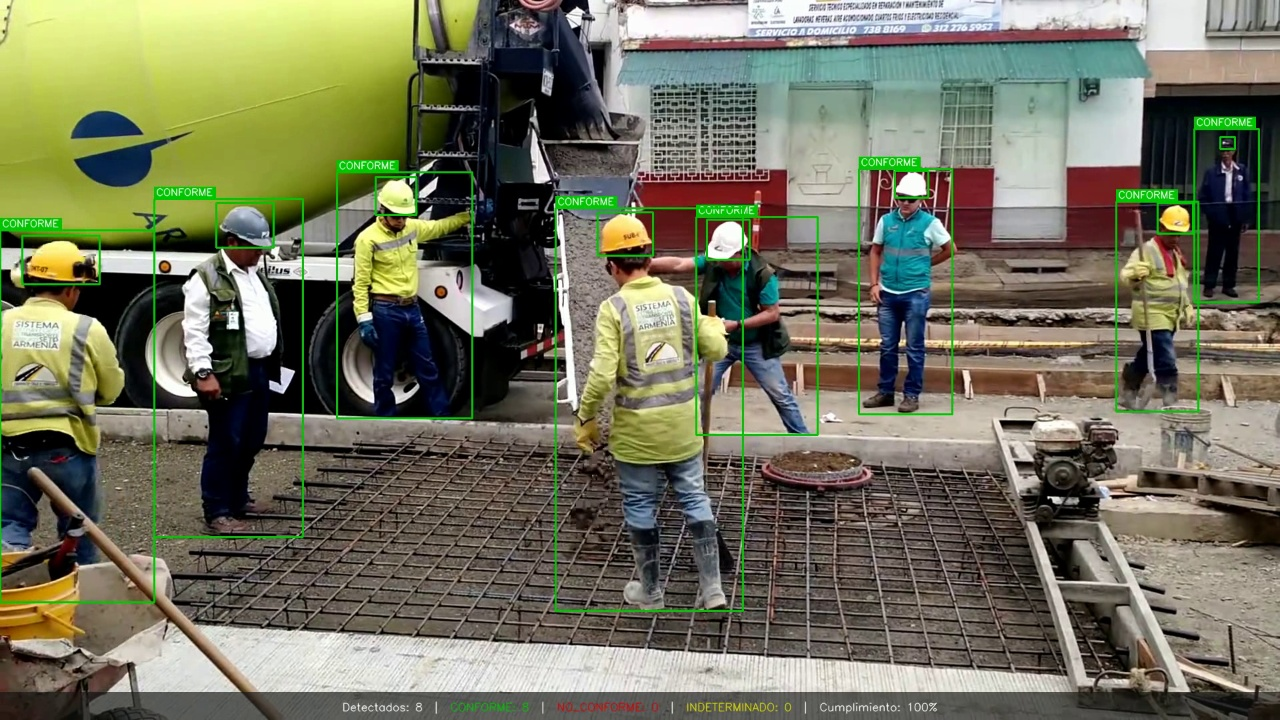
\includegraphics[width=\linewidth]{figures/demo_finetuned.jpg}
    \caption{Fine-tuned}
\end{subfigure}
\caption{Mismo fotograma de \texttt{video03p.mp4} procesado por
las tres versiones del sistema. El modelo \textit{fine-tuned}
cubre escena completa con un solo modelo.}
\label{fig:demos}
\end{figure*}

% ============================================================
\section{Implicaciones éticas}
% ============================================================

\subsection{Asimetría entre falsos negativos y positivos}

Los dos tipos de error tienen costos asimétricos: un falso negativo
deja al trabajador en riesgo; un falso positivo erosiona la
confianza en el sistema. \textbf{En seguridad ocupacional, el falso
negativo es típicamente más costoso}. El umbral del clasificador no
debe elegirse maximizando mAP global sino considerando el costo
asimétrico de los errores. El estado INDETERMINADO funciona como
\emph{mecanismo de seguridad}: el sistema no inventa veredictos.

\subsection{Privacidad}

Un sistema que graba continuamente plantea cuestiones de
vigilancia, uso secundario de imágenes y consentimiento informado.
El sistema técnico no resuelve esto por sí solo: requiere
anonimización de rostros, retención mínima necesaria, acceso
restringido por roles y auditoría de uso.

\subsection{Sesgos del dataset}

Los datasets utilizados tienen sesgos identificables: geográfico
(dominio China/EE.UU./Europa), demográfico (distribución no
auditada) y de captura (iluminación diurna, clima despejado). Las
métricas reportadas son válidas para la distribución del test set;
no son garantía sobre condiciones de despliegue distintas.

% ============================================================
\section{Limitaciones y trabajo futuro}
% ============================================================

Limitaciones: sesgo de etiquetado entre datasets, clase
\texttt{person} históricamente escasa (atacada vía fine-tuning),
Experimento A (resolución 960) no evaluado, grupo de oclusión
alta estadísticamente débil ($n=15$), sin auditoría de sesgos
demográficos, sin tracking temporal entre frames.

Trabajo futuro: modelo más grande (YOLOv8m o YOLOv9), resolución
de inferencia 1600+, tracking temporal con ByteTrack, calibración
del umbral según costo asimétrico, detección de arnés para trabajos
en altura.

% ============================================================
\section{Conclusiones}
% ============================================================

\begin{enumerate}
    \item Detector YOLOv8s entrenado con \textbf{mAP@0.5 = 0.771}
    sobre test no visto, con desempeño excelente en las tres clases
    críticas (todas $\geq 0.947$).

    \item El modelo \textbf{generaliza correctamente}: val vs test
    prácticamente idénticos ($-0.4$~pp).

    \item Verificador determinista validado con 39 tests pytest
    pasando + inspección cualitativa sobre val y video real.

    \item Limitación estructural diagnosticada (sesgo de etiquetado,
    3.3\% de coocurrencia) y \textbf{validada experimentalmente}
    contra un modelo externo ($2.75\times$ más veredictos
    definitivos).

    \item Dos mejoras iterativas aplicadas: \emph{pipeline} híbrido
    (cobertura $\times 1.67$) y \emph{fine-tuning} sobre OtroEnfoque
    (clase \texttt{person} de $0.17$ a $0.71$, $+302\%$).

    \item Sistema con \emph{calibración honesta de incertidumbre}
    mediante INDETERMINADO; no alucina veredictos sin evidencia.

    \item Tres ejes éticos identificados (asimetría de errores,
    privacidad, sesgos) cuya resolución requiere políticas
    operativas además del sistema técnico.
\end{enumerate}

% ============================================================
% Bibliografía
% ============================================================
\begin{thebibliography}{99}

\bibitem{ultralytics2023}
G. Jocher, A. Chaurasia, and J. Qiu,
``YOLO by Ultralytics,''
\url{https://github.com/ultralytics/ultralytics}, 2023.

\bibitem{redmon2016}
J. Redmon, S. Divvala, R. Girshick, and A. Farhadi,
``You Only Look Once: Unified, Real-Time Object Detection,''
\emph{Proc. IEEE Conf. Computer Vision and Pattern Recognition
(CVPR)}, pp. 779--788, 2016.

\bibitem{roboflow}
Roboflow Universe,
``Open source computer vision datasets and pre-trained models,''
\url{https://universe.roboflow.com}, 2024.

\bibitem{shwd}
njvisionpower,
``Safety Helmet Wearing Dataset (SHWD),''
\url{https://github.com/njvisionpower/Safety-Helmet-Wearing-Dataset},
2019.

\bibitem{cocometrics}
T.-Y. Lin et al.,
``Microsoft COCO: Common Objects in Context,''
\emph{Proc. European Conf. Computer Vision (ECCV)}, pp. 740--755,
2014.

\bibitem{supervision}
Roboflow,
``Supervision: tools for computer vision,''
\url{https://github.com/roboflow/supervision}, 2023.

\bibitem{snehilcss}
S. Sanyal,
``Construction Site Safety Image Dataset,''
Roboflow Universe / Kaggle, 2023.

\end{thebibliography}

\end{document}
